Encuentra el valor de la incógnita en el triángulo de la figura \ref{fig:angle_triangle_12}.

\begin{minipage}[t][4cm][b]{0.3\textwidth}
    \begin{figure}[H]
        \centering
        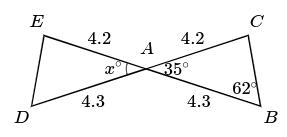
\includegraphics[width=0.99\linewidth]{../images/angle_triangle_12.png}
        \caption{}
        \label{fig:angle_triangle_12}
    \end{figure}
\end{minipage}\hfill
\begin{minipage}[t]{0.65\textwidth}
    \begin{solutionbox}{4cm}
        $\angle DAE$ forma un ángulo opuesto por el vértice con $\angle BAC$.\\
        \[\Rightarrow \angle DAE = \angle BAC \]
        Observamos que el ángulo $x$ corresponde al
        $\angle BAC$ y $\angle BAC$ mide
        35$^\circ$.
        \[\therefore x=35^\circ\]
    \end{solutionbox}
\end{minipage}
